\documentclass[innermargin=10mm]{tikzposter} % See Section 3
\usepackage{enumitem}
\usepackage{url}
\usepackage{wrapfig}
\usepackage{textcomp}
\usepackage{enumitem}
\geometry{paperwidth=63in,paperheight=42in}
\graphicspath{./images/}

\title{Learning topography with Tangible Landscape games}
\institute{$^1$North Carolina State University, Raleigh, NC, USA (\texttt{akratoc@ncsu.edu}),
$^2$Louisiana State University, Baton Rouge, LA, USA}
\author{Anna Petrasova$^1$, Payam Tabrizian$^1$, Brendan A. Harmon$^2$,\\ Vaclav Petras$^1$,
Garrett Millar$^1$, Helena Mitasova$^1$ and Ross K. Meentemeyer$^1$}
% \titlegraphic{\includegraphics{./images/logos/ncstate-type-2x2-red-rgb.eps}}

\usetheme{Rays} % See Section 5
%  \usebackgroundstyle{Autumn}
% \usetitlestyle{Rays}




\renewcommand{\familydefault}{\sfdefault}


\definecolor{mybrown}{HTML}{58433C}
\definecolor{mybrown2}{HTML}{8B7168}

\definecolor{gr1}{HTML}{F0F0F0}
\definecolor{gr2}{HTML}{D6E6C2}


\definecolorstyle{test} {
\definecolor{colorOne}{named}{white}
\definecolor{colorTwo}{named}{mybrown}
\definecolor{colorThree}{named}{mybrown2}
}{
\colorlet{titlebgcolor}{colorOne}
\colorlet{titlefgcolor}{colorTwo}
\colorlet{framecolor}{white}
}

\definecolor{textcolor}{HTML}{000000}
\definecolor{titleTextColor}{HTML}{009000}
\definecolorpalette{grassColorPalette} {
  \definecolor{colorOne}{HTML}{419041}
  % \definecolor{colorTwo}{HTML}{cccccc}
  \definecolor{colorTwo}{HTML}{dddddd}
  \definecolor{colorThree}{HTML}{F1B52D}
  % \definecolor{colorThree}{HTML}{EFA126}
}

\definecolorpalette{or} {
  \definecolor{colorOne}{HTML}{4C923F}
  \definecolor{colorTwo}{HTML}{dddddd}
  \definecolor{colorThree}{HTML}{36672D}
}



% \usecolorstyle{test}
\usecolorstyle[colorPalette=or]{Britain}

\colorlet{blocktitlefgcolor}{colorThree}
% \usenotestyle{Corner}





\makeatletter
\renewcommand\TP@maketitle{%
    \begin{minipage}{0.15\linewidth}
       \centering
       \includegraphics[width=0.8\textwidth]{./images/cgaNCSU}
    \end{minipage}%
    \hfill
   \begin{minipage}{0.7\linewidth}
        \centering
        \color{titlefgcolor}
        {\bfseries  \sc {\fontsize{95}{60}\selectfont \@title}  \par}
        \vspace*{1em}
        {\huge \@author \par}
        \vspace*{1em}
        {\LARGE \@institute}
    \end{minipage}%
    \hfill
    \begin{minipage}{0.15\linewidth}
      \centering
%        \includegraphics[width=0.37\textwidth]{grass_logo.pdf}\\
      \includegraphics[width=0.65\textwidth]{./images/tl_logo.pdf}\\
%       \Large {\textsf{GRASS GIS}}
   \end{minipage}
%     \begin{minipage}{0.2\linewidth}
%        \centering
%        \includegraphics[width=0.45\textwidth]{./images/logos/grass_logo.pdf}
%     \end{minipage}
}
\makeatother
\makeatletter
\setlength{\TP@visibletextwidth}{\textwidth-3\TP@innermargin}
\setlength{\TP@visibletextheight}{\textheight-3\TP@innermargin}
\makeatother

\newcommand{\seeanimtext}{see animation online}%
\newcommand{\blocktitlesize}{\huge }


\setlength{\parskip}{1cm}

\begin{document}
\maketitle[width=0.8\textwidth,roundedcorners=30pt] % See Section 4.1


\begin{columns} % See Section 4.4
\column{0.25} % See Section 4.4
\block[titleleft,titleinnersep=8mm]{\blocktitlesize Introduction}{
\setlength{\parskip}{1em}
\vspace{-20pt}
\LARGE


\begin{wrapfigure}[10]{L}{0.6\linewidth}
\vspace{-20pt}
\includegraphics[width=0.95\linewidth]{./images/interaction}
\end{wrapfigure}
We developed and tested a new method for teaching hydrology, geomorphology,
and grading using Tangible Landscape\,---\,a tangible interface for geospatial modeling.
Tangible Landscape couples a physical and digital model of a landscape through
a real-time cycle of hands-on modeling, 3D scanning, geospatial computation,
and projection.
With Tangible Landscape students can: %sculpt a projection-augmented
% topographic model of a landscape with their hands and use a variety of tangible objects
% to immediately see how they are changing geospatial analytics such as contours, profiles,
% water flow, or landform types. By feeling and manipulating the shape of the topography,
% while seeing projected geospatial analytics, students can intuitively learn about 3D topographic form,
% its representations, and how topography controls physical processes.
\begin{itemize}[leftmargin=1.5cm]
 \item[\textbullet{} ] feel and manipulate the shape of topography with their hands
 and use a variety of tangible objects
 \item[\textbullet{} ] sculpt a projection-augmented topographic model of a landscape while seeing dynamically computed projected geospatial analytics
 \item[\textbullet{} ] intuitively learn about 3D topographic form, its representations, and how topography controls physical processes
\end{itemize}

\begin{center}
\includegraphics[width=0.865\linewidth]{./images/TL_Setup}
\end{center}

Tangible Landscape powered by GRASS GIS,
an open source platform with extensive libraries for geospatial modeling,
can be flexibly programmed to accommodate simple to complex
geospatial applications and simulations, thus providing a
broader range of teaching opportunities than preceding geospatial tangible user interfaces (TUI).

}




\column{0.5}
\block[titleleft,titleinnersep=8mm]{\blocktitlesize Tangible Landscape games}
{

\LARGE
Students of a graduate level course on grading  participated in a series of workshops,
which were developed as serious games to encourage learning through structured play.
The games focused on hydrology, geomorphology, and grading concepts.

\vspace{1em}

\begin{minipage}{1\linewidth}
\begin{minipage}{0.45\linewidth}
\setlength{\parskip}{0pt plus 0pt minus 0pt}
%width,linewidth,roundedcorners
%
% \rule{0em}{1em}
\vspace{2em}
\coloredbox[bgcolor=gr1,framecolor=gr1,roundedcorners=15]{
\textbf{Water flow task:}
Find the highest source point from which water will
flow into the target point in the landscape.
Mark the location of the source
point location by inserting a wooden pin into the model.
}


\vspace{2.8em}

\coloredbox[bgcolor=gr1,framecolor=gr1,roundedcorners=15]{
\textbf{Channeling task:}
Modify the terrain with minimal changes to
make water flow from the given source point to the given
target point. Use your hands or sculpting knife
to shape the topography.
}


\vspace{2.7em}

\coloredbox[bgcolor=gr1,framecolor=gr1,roundedcorners=15]{
\textbf{Ponding task:}
With the given amount of sand and the existing topography build
a damn on a stream to impound maximum volume of water.
Use your hands or sculpting knife to make dams in the landscape.
}

\vspace{2.7em}

\coloredbox[bgcolor=gr1,framecolor=gr1,roundedcorners=15]{
\textbf{Landform task:}
With your hands sculpt combinations of specified landforms (depressions, ridges, valleys, peaks)
and identify them. The combinations get increasingly difficult.
}

\vspace{2em}

\coloredbox[bgcolor=gr1,framecolor=gr1,roundedcorners=15]{
\textbf{Simple cut \& fill task:}
Modify a given landscape using dynamically computed cut and fill projection, where
blue indicates the areas where sand
should be added (fill), red indicates where sand
should be removed (cut), and the color intensity
indicates the magnitude of the difference.
}

\vspace{1.5em}

\coloredbox[bgcolor=gr1,framecolor=gr1,roundedcorners=15]{
\textbf{Advanced cut \& fill task:}
Modify existing topography in highlighted areas to match the projected
contours and color by removing or adding sand. 
The indicator shows the total elevation
difference between the scanned model and the expected topography.
}

% \vspace{1em}
\end{minipage}
\hfill
\begin{minipage}{0.53\linewidth}
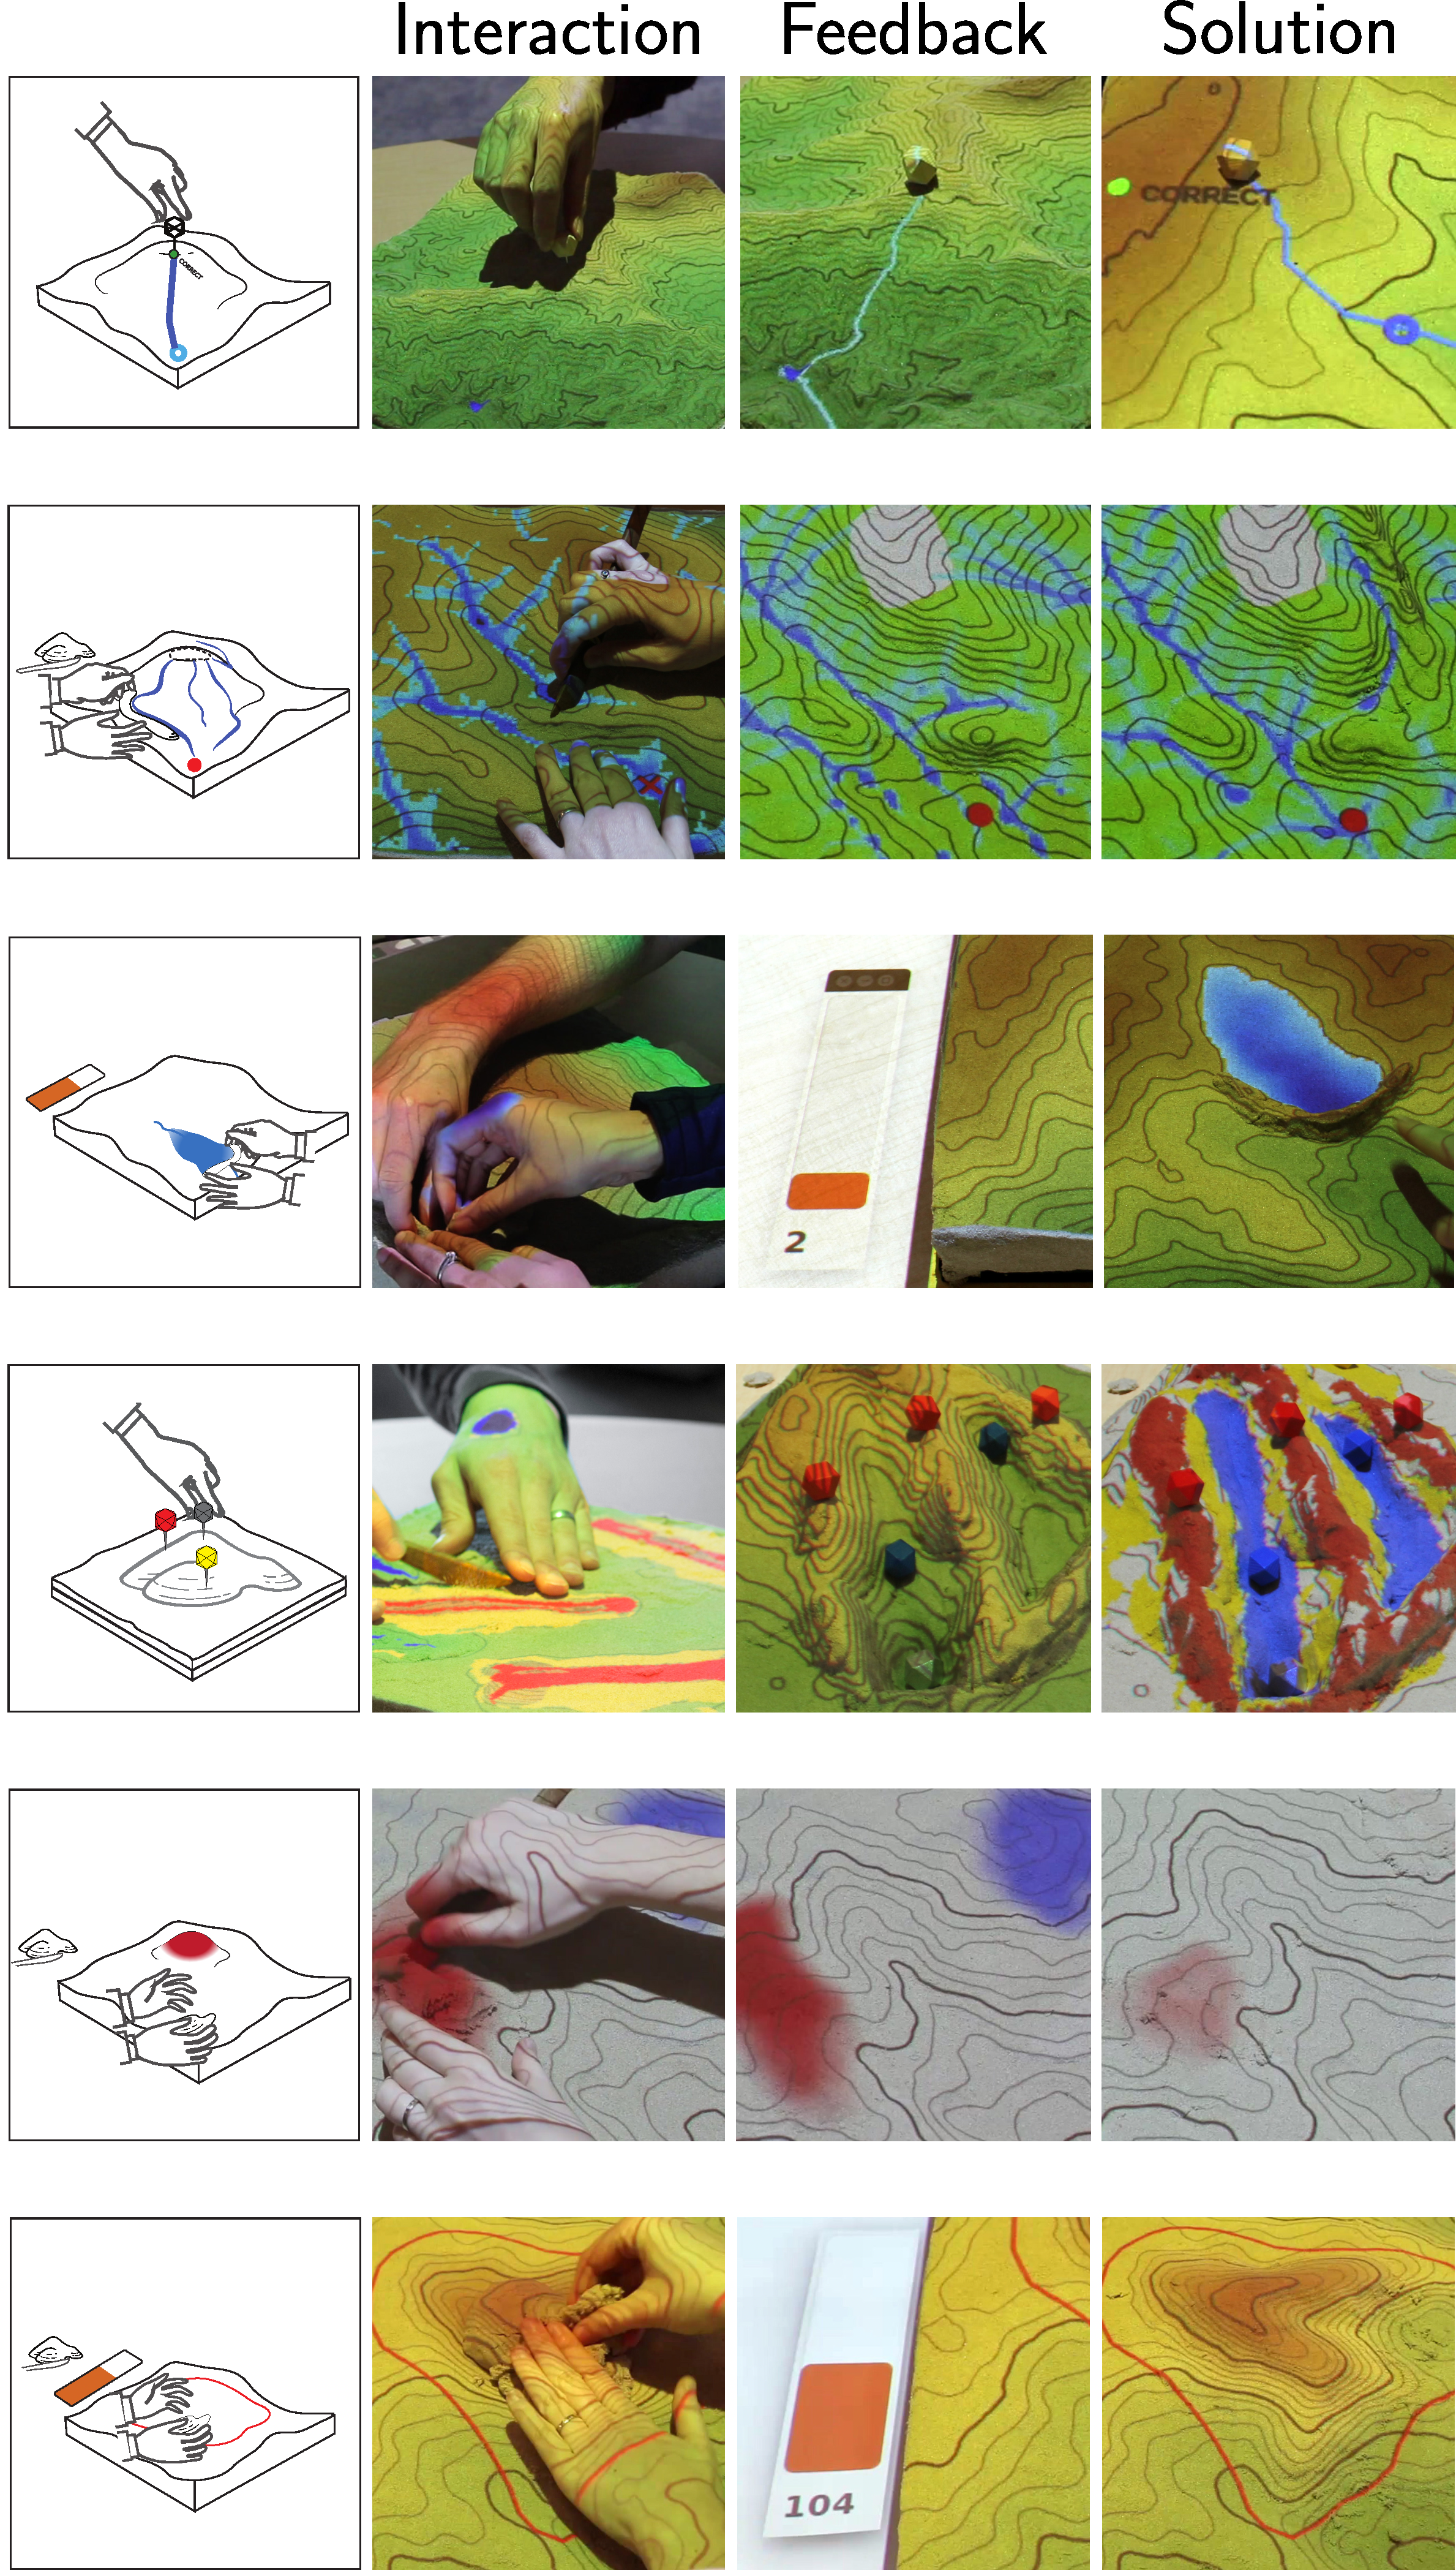
\includegraphics[width=1\linewidth]{./images/games}
\end{minipage}
\end{minipage}

\vspace{2.1em}

The geospatial analyses displayed as feedback are implemented in the following GRASS GIS modules:
r.drain (flow routing), r.sim.water (flow simulation), r.fill.dir (elevation depressions),
r.geomorphon (landforms), r.mapcalc (elevation difference).


% \raisebox{0pt}[0pt][0pt]{\hspace{-3cm}\colorbox{white}{\includegraphics[width=3cm]{images/qrcodes/youtube1}}}%
\newlength{\myl}%
\settowidth{\myl}{\tiny\seeanimtext}%
% \raisebox{-1ex}[0pt][0pt]{\hspace{-1.8\myl}\colorbox{white}{\small\seeanimtext}}

}



\column{0.25}
\block[titleleft,titleinnersep=8mm]{\blocktitlesize Pilot user study}{
\LARGE
% 
\begin{description}[leftmargin=0cm]
 \item[Goal ]
 Test the effectiveness of a tangible teaching method\,---\,implemented with Tangible Landscape\,---\,for
 teaching concepts of grading, geomorphology, and hydrology.
 \item[Subjects ] 16 graduate students from a Landform and Grading course in the Department of Landscape Architecture
%  participated in three sessions
\item[Assessment]~\\%We assessed the effectiveness of Tangible Landscape as a teaching tool through: 
\vspace{-1.5em}
\begin{itemize}[leftmargin=1.5cm]
 \item[\textbullet{} ] Usability and user experience (UX) survey designed and validated for geospatial TUIs,
 
 \item[\textbullet{} ] Three assessments administered before and after workshops to assess acquisition
 and transfer of spatial skills: topographic map assessment (TMA) and  two assessments specific to landforms and cut \& fill tasks
%  \item[\textbullet{} ] topographic map assessment (TMA) to assess acquisition and transfer of spatial skills
%  \item[\textbullet{} ] two assessments specific to landforms and cut and fill tasks
\end{itemize}
% \begin{center}
\vspace{0.2em}
\begin{minipage}{0.85\linewidth}
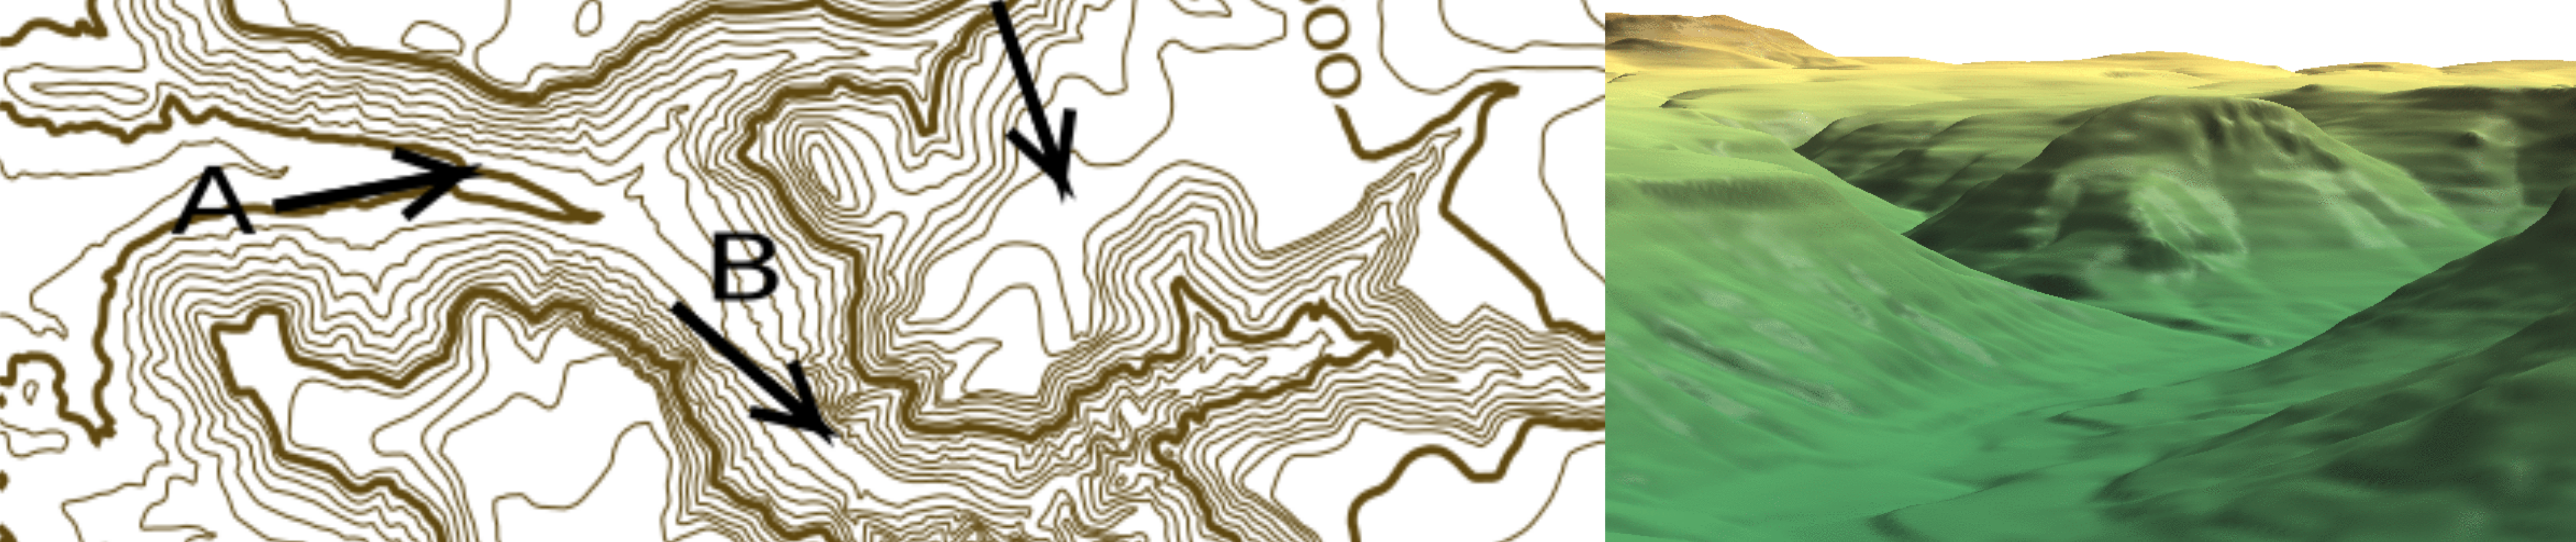
\includegraphics[width=1\linewidth]{./images/tma}
\end{minipage}
%
\begin{minipage}{0.14\linewidth}
\fontsize{27}{30.} \selectfont TMA\\ example task
\end{minipage}

\vspace{0.5em}
% \end{center}
\item[Results ]
Findings provide evidence that Tangible Landscape supports 
improved UX and marginal, task-specific knowledge building.
\begin{itemize}[leftmargin=1.5cm]
 \item[\textbullet{} ] The objects' physicality enabled
participants to effectively interact with the system,
positively impacting ratings of the system's usability and UX.
\item[\textbullet{} ] No significant response accuracy differences for TMA nor landform assessment,
potentially due to mismatched psychometric properties of examining tangible (3D)
teaching methods with 2D assessments of learning outcomes.
 \item[\textbullet{} ] Students scored significantly better on the cut and fill assessment after workshop, in comparison to before.
\end{itemize}


\end{description}


\setlength{\parskip}{0.5cm}
\LARGE

}

\block[titleleft,titleinnersep=8mm]{\blocktitlesize Additional resources}{
% qrcode -t EPS -o testing_doc.eps "www.youtube.com/watch?v=QBPzYXiL3TY"

\begin{description}
\item[Tangible Landscape ] \url{github.com/tangible-landscape}
\item[User survey and TMA ] \url{osf.io/b6njq}
 \item[NCSU GeoForAll Lab ] \url{geospatial.ncsu.edu/osgeorel}
 
\end{description}

}

\block[titleleft]{\blocktitlesize References \& Acknowledgement}{
\fontsize{27}{37.} \selectfont
\begin{enumerate}[label={[\arabic*]}]
 \item Petrasova, A., Harmon, B. A., Petras, V., Mitasova, H., 2015.
\emph{Tangible Modeling with Open Source GIS.}
Springer International Publishing, 135 p.% DOI: 10.1007/978-3-319-25775-4


\item Neteler, M., Bowman, M. H., Landa, M., Metz, M., 2012.
\emph{GRASS GIS: A multi-purpose open source GIS.}
Environmental Modelling \& Software, 31(0), 124--130.

\end{enumerate}

\bigskip

This research was partially supported through 
\textbf{GAPS (Geospatial Analytics for Problem Solving) for Hi-Tech Teens} program funded by
Burroughs Wellcome Fund
}
\end{columns}
\end{document}